\XtoCBlock{TF1}
\label{block:TF1}
\begin{figure}[H]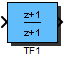
\includegraphics{TF1}\end{figure} 

\begin{XtoCtabular}{Inports}
In & Input In(k)\tabularnewline
\hline
\end{XtoCtabular}


\begin{XtoCtabular}{Outports}
Out & Output Out(k)\tabularnewline
\hline
\end{XtoCtabular}

\begin{XtoCtabular}{Mask Parameters}
b1 & b1\tabularnewline
\hline
b0 & b0\tabularnewline
\hline
a0 & a0\tabularnewline
\hline
ts\_fact & Multiplication factor of base sampling time (in integer format)\tabularnewline
\hline
\end{XtoCtabular}

\subsubsection*{Description:}
First order transfer function:

    G(z) = (b1.z + b0) / (z + a0)

% include optional documentation file
\InputIfFileExists{\XcHomePath/Library/Control/Doc/TF1_Info.tex}{\vspace{1ex}}{}

\subsubsection*{Implementations:}
\begin{tabular}{l l}
\textbf{FiP8} & 8 Bit Fixed Point Implementation\tabularnewline
\textbf{FiP16} & 16 Bit Fixed Point Implementation\tabularnewline
\textbf{FiP32} & 32 Bit Fixed Point Implementation\tabularnewline
\textbf{Float32} & 32 Bit Floating Point Implementation\tabularnewline
\textbf{Float64} & 64 Bit Floating Point Implementation\tabularnewline
\end{tabular}

\XtoCImplementation{FiP8}
\index{Block ID!3280}
\nopagebreak[0]
% Implementation details
\begin{tabular}{l l}
\textbf{Name} & FiP8 \tabularnewline
\textbf{ID} & 3280 \tabularnewline
\textbf{Revision} & 0.1 \tabularnewline
\textbf{C filename} & TF1\_FiP8.c \tabularnewline
\textbf{H filename} & TF1\_FiP8.h \tabularnewline
\end{tabular}
\vspace{1ex}

8 Bit Fixed Point Implementation

\begin{XtoCtabular}{Controller Parameters}
b0 & Coefficient b0\tabularnewline
\hline
b1 & Coefficient b1\tabularnewline
\hline
a0 & Coefficient a0\tabularnewline
\hline
sfrb & Shift factor for coefficient b0 and b1\tabularnewline
\hline
sfra & Shift factor for coefficient a0\tabularnewline
\hline
in\_old & In(k-1)\tabularnewline
\hline
\end{XtoCtabular}

% Implementation data structure
\XtoCDataStruct{Data Structure:}
\begin{lstlisting}
typedef struct {
     uint16        ID;
     int8          *In;
     int8          Out;
     int8          b0;
     int8          b1;
     int8          a0;
     int8          sfrb;
     int8          sfra;
     int8          in_old;
} TF1_FIP8;
\end{lstlisting}

\ifdefined \AddTestReports
\InputIfFileExists{\XcHomePath/Library/Control/Doc/Test_TF1_FiP8.tex}{}{}
\fi
\XtoCImplementation{FiP16}
\index{Block ID!3281}
\nopagebreak[0]
% Implementation details
\begin{tabular}{l l}
\textbf{Name} & FiP16 \tabularnewline
\textbf{ID} & 3281 \tabularnewline
\textbf{Revision} & 0.1 \tabularnewline
\textbf{C filename} & TF1\_FiP16.c \tabularnewline
\textbf{H filename} & TF1\_FiP16.h \tabularnewline
\end{tabular}
\vspace{1ex}

16 Bit Fixed Point Implementation

\begin{XtoCtabular}{Controller Parameters}
b0 & Coefficient b0\tabularnewline
\hline
b1 & Coefficient b1\tabularnewline
\hline
a0 & Coefficient a0\tabularnewline
\hline
sfrb & Shift factor for coefficient b0 and b1\tabularnewline
\hline
sfra & Shift factor for coefficient a0\tabularnewline
\hline
in\_old & In(k-1)\tabularnewline
\hline
\end{XtoCtabular}

% Implementation data structure
\XtoCDataStruct{Data Structure:}
\begin{lstlisting}
typedef struct {
     uint16        ID;
     int16         *In;
     int16         Out;
     int16         b0;
     int16         b1;
     int16         a0;
     int8          sfrb;
     int8          sfra;
     int16         in_old;
} TF1_FIP16;
\end{lstlisting}

\ifdefined \AddTestReports
\InputIfFileExists{\XcHomePath/Library/Control/Doc/Test_TF1_FiP16.tex}{}{}
\fi
\XtoCImplementation{FiP32}
\index{Block ID!3282}
\nopagebreak[0]
% Implementation details
\begin{tabular}{l l}
\textbf{Name} & FiP32 \tabularnewline
\textbf{ID} & 3282 \tabularnewline
\textbf{Revision} & 0.1 \tabularnewline
\textbf{C filename} & TF1\_FiP32.c \tabularnewline
\textbf{H filename} & TF1\_FiP32.h \tabularnewline
\end{tabular}
\vspace{1ex}

32 Bit Fixed Point Implementation

\begin{XtoCtabular}{Controller Parameters}
b0 & Coefficient b0\tabularnewline
\hline
b1 & Coefficient b1\tabularnewline
\hline
a0 & Coefficient a0\tabularnewline
\hline
sfrb & Shift factor for coefficient b0 and b1\tabularnewline
\hline
sfra & Shift factor for coefficient a0\tabularnewline
\hline
in\_old & In(k-1)\tabularnewline
\hline
\end{XtoCtabular}

% Implementation data structure
\XtoCDataStruct{Data Structure:}
\begin{lstlisting}
typedef struct {
     uint16        ID;
     int32         *In;
     int32         Out;
     int32         b0;
     int32         b1;
     int32         a0;
     int8          sfrb;
     int8          sfra;
     int32         in_old;
} TF1_FIP32;
\end{lstlisting}

\ifdefined \AddTestReports
\InputIfFileExists{\XcHomePath/Library/Control/Doc/Test_TF1_FiP32.tex}{}{}
\fi
\XtoCImplementation{Float32}
\index{Block ID!3283}
\nopagebreak[0]
% Implementation details
\begin{tabular}{l l}
\textbf{Name} & Float32 \tabularnewline
\textbf{ID} & 3283 \tabularnewline
\textbf{Revision} & 0.1 \tabularnewline
\textbf{C filename} & TF1\_Float32.c \tabularnewline
\textbf{H filename} & TF1\_Float32.h \tabularnewline
\end{tabular}
\vspace{1ex}

32 Bit Floating Point Implementation

\begin{XtoCtabular}{Controller Parameters}
b0 & Coefficient b0\tabularnewline
\hline
b1 & Coefficient b1\tabularnewline
\hline
a0 & Coefficient a0\tabularnewline
\hline
in\_old & In(k-1)\tabularnewline
\hline
\end{XtoCtabular}

% Implementation data structure
\XtoCDataStruct{Data Structure:}
\begin{lstlisting}
typedef struct {
     uint16        ID;
     float32       *In;
     float32       Out;
     float32       b0;
     float32       b1;
     float32       a0;
     float32       in_old;
} TF1_FLOAT32;
\end{lstlisting}

\ifdefined \AddTestReports
\InputIfFileExists{\XcHomePath/Library/Control/Doc/Test_TF1_Float32.tex}{}{}
\fi
\XtoCImplementation{Float64}
\index{Block ID!3284}
\nopagebreak[0]
% Implementation details
\begin{tabular}{l l}
\textbf{Name} & Float64 \tabularnewline
\textbf{ID} & 3284 \tabularnewline
\textbf{Revision} & 0.1 \tabularnewline
\textbf{C filename} & TF1\_Float64.c \tabularnewline
\textbf{H filename} & TF1\_Float64.h \tabularnewline
\end{tabular}
\vspace{1ex}

64 Bit Floating Point Implementation

\begin{XtoCtabular}{Controller Parameters}
b0 & Coefficient b0\tabularnewline
\hline
b1 & Coefficient b1\tabularnewline
\hline
a0 & Coefficient a0\tabularnewline
\hline
in\_old & In(k-1)\tabularnewline
\hline
\end{XtoCtabular}

% Implementation data structure
\XtoCDataStruct{Data Structure:}
\begin{lstlisting}
typedef struct {
     uint16        ID;
     float64       *In;
     float64       Out;
     float64       b0;
     float64       b1;
     float64       a0;
     float64       in_old;
} TF1_FLOAT64;
\end{lstlisting}

\ifdefined \AddTestReports
\InputIfFileExists{\XcHomePath/Library/Control/Doc/Test_TF1_Float64.tex}{}{}
\fi
